\documentclass[a4paper,titlepage,openright,12pt]{report}
\usepackage{graphicx}    
%\usepackage{epsfig}   
\usepackage[font=footnotesize]{subfig}
\usepackage{float}
\usepackage{fancyhdr}                              
\usepackage{makeidx}
\usepackage[nottoc,notlot,notlof]{tocbibind}     
\usepackage{supertabular}
\usepackage{array}              
\usepackage{setspace} 
\usepackage{enumerate}
\usepackage{rotating}
\usepackage{moreverb}
\usepackage{multirow}
\usepackage{amsmath}
\usepackage{amsthm}
\usepackage{amssymb}
\usepackage{captcont}
\usepackage{verbatim}
\usepackage{titlesec}
\usepackage{url}
\usepackage{hyperref}
\usepackage{lipsum}
\usepackage{tabularx}
\usepackage{url}
%\usepackage[algoruled]{algorithm2e}
%\usepackage[figure,algoruled]{algorithm2e}
%\usepackage[figure,boxruled]{algorithm2e}

%\newtheorem{theorem}{Theorem}
%\newtheorem{corollary}[theorem]{Corollary}
%\newtheorem{conjecture}[theorem]{Conjecture}
%\newtheorem{lemma}[theorem]{Lemma}
%\newtheorem{proposition}[theorem]{Proposition}
%\newtheorem{definition}[theorem]{Definition}
%\newtheorem{Example}[theorem]{Example}
%\newtheorem{axiom}{Axiom}
%\newtheorem{remark}{Remark}
%\newtheorem{exercise}{Exercise}[section]
%\newtheorem{fact}[theorem]{Fact}
%\newtheorem{property}[theorem]{Property}
\setlength{\parindent}{0pt}%for paragraph spacing
\setlength{\parskip}{1ex plus 0.5ex minus 0.2ex}
\setlength{\textheight}{8.5in}
\pagestyle{fancy}
% with this we ensure that the chapter and section
% headings are in lowercase.
%\renewcommand{\bibname}{References}
\renewcommand{\chaptermark}[1]{\markboth{#1}{}}
\renewcommand{\sectionmark}[1]{\markright{\thesection\ #1}}
\fancyhf{} % delete current setting for header and footer
\fancyhead[LE,RO]{\bfseries\thepage}
\fancyhead[LO]{\bfseries\rightmark}
\fancyhead[RE]{\bfseries\leftmark}
%\rfoot{\bfseries\thepage}
\cfoot{\em $\copyright$ 2015-16, Indian Institute of Technology Delhi}
\renewcommand{\headrulewidth}{0.5pt}
\renewcommand{\footrulewidth}{0.5pt}
\addtolength{\headheight}{2.5pt} % make space for the rule

\fancypagestyle{plain}{%
\fancyhead{} % get rid of headers on plain pages
\fancyfoot{}
%\rfoot{\bfseries\thepage}
\cfoot{\em $\copyright$ 2015-16, Indian Institute of Technology Delhi}
\renewcommand{\headrulewidth}{0pt} % and the line
}

%% The smart version of cleardouble page.
\let\origdoublepage\cleardoublepage
\newcommand{\clearemptydoublepage}{%
  \clearpage
  {\pagestyle{empty}\origdoublepage}%
}

\let\cleardoublepage\clearemptydoublepage


\date{}


\addtolength{\oddsidemargin}{30pt}
\addtolength{\evensidemargin}{-40pt}

\titlespacing*{\chapter}{0pt}{-50pt}{20pt}
\titleformat{\chapter}[display]{\normalfont\huge\bfseries}{\chaptertitlename\ \thechapter}{20pt}{\Huge}
% \DeclareGraphicsExtensions{.pdf,.png,.jpg,.ps}
\floatstyle{boxed} 
\restylefloat{figure}
\setcounter{lofdepth}{2}
\setcounter{lotdepth}{2}

\newtheorem{claim}{Claim}[section]
\newtheorem{theorem}{Theorem}[section]
\newtheorem{defn}{Definition}[section]
\newtheorem{fact}{Fact}[section]

\graphicspath{{./Figures/}}
\begin{document}

%\begin{comment}
% Begin title page
\begin{titlepage}
\begin{center}

\LARGE{\textsf{\bfseries The Corporate-Political Nexus}}\\
\vspace{20pt}
\normalsize
\emph{A thesis submitted in fulfillment} \\
\emph{of the requirements for} \\
\vspace{20pt}
\bfseries M.TECH MAJOR PROJECT \\
%\vspace{20pt}
%\emph {in}\\
%\vspace{20pt}
%\bfseries Deptartment of Computer Science \& Engineering \\
%\vspace{20pt}
\emph {by}\\
\vspace{20pt}
\Large{\textsf{\bfseries ABHISHEK AGARWAL}} \\
{\normalsize \textsf{\bfseries Entry No. 2014MCS2114}}\\

\ \\
%\ \\
{\normalsize \emph {Under the guidance of}}
\ \\
\Large{\textsf{\bfseries Dr. AADITESHWAR SETH}} \\
\ \\
\vspace{30pt}
%\begin{center}

\includegraphics[scale=0.2]{iit_logo.pdf} \\
\vspace{10pt}
%\end{center}
\large{\textsc{Department of Computer Science and Engineering,\\
Indian Institute of Technology Delhi.\\ June 2016.}}
\end{center}
\end{titlepage}

%\newpage
%\cleardoublepage
\onehalfspacing
\thispagestyle{empty}

\normalfont
\begin{center}
\LARGE{ Certificate}
\end{center}

\vspace{0.5in}

This is to certify that the thesis titled {\bfseries The Corporate-Political Nexus} being submitted by
{\bfseries AMARTYA CHAUDHURI} for the award of {\bfseries Master of Technology} in {\bfseries Computer Science \& Engineering} is a record of bona fide work carried out by him under my guidance and supervision at the {\bfseries Department of Computer Science \& Engineering}. The work presented in this thesis has not been submitted elsewhere either in part or full, for the award of any other degree or diploma.

\vspace{1.5in}


{\bfseries Dr. AADITESHWAR SETH} \\
{\bfseries Department of Computer Science and Engineering} \\
{\bfseries Indian Institute of Technology, Delhi}\\

\thispagestyle{empty}
%\begin{center}
\LARGE{Acknowledgments}  %This is the correct spelling dont change sit
\end{center}

\vspace{0.5in}

%Replace \lipsum with your acknowledgement
%\lipsum[1]
I would like to express my heartiest gratitude to my supervisor Dr. Aaditeshwar Seth for guiding this work with utmost interest and scientific rigor. I thank him for setting high standards, giving me freedom to explore multiple facets of the problem and teaching me the value of analytical thinking and hard work. I am also grateful to Manoj Kumar, Anirban Sen and Dipanjan Chakraborty who have helped a great deal by providing their support during difficult times and whose suggestions went a long way in making this work a reality. I am highly indebted to Preeti Rani, Mridul Goel and Md. Imran for actually sitting with me and working on perfecting the final system. I would also like to thank my family and friends for their love and support and bearing with me for my constant absence.\\

\vspace{1.5in}

{\bfseries ABHISHEK AGARWAL}


\thispagestyle{empty}


% \setcounter{page}{1}
% \pagenumbering{roman}
\thispagestyle{empty}
\begin{center}
\LARGE{Abstract}
\end{center}

\vspace{0.5in}

%replace \lipsum with your abstract
%\lipsum[1]
In this project we try to facilitate the study of distribution of power across and within various Indian power institutions by analysing their inter-linkages, family trees, timelines, transactions, etc. to make more sense of the big political and corporate handshakes. In that direction, we envision to construct a system to collect data in this regard from various sources and integrate all of it into a single data store for others to use.

Our aim is to disseminate these findings to the mass society using a crowdsourced system, and use mass language for such a flow of information. and in this way, enhance governmental accountability and transparency using the notion of Open data and crowdsourcing.



\thispagestyle{empty}
\begin{center}
\LARGE{Acknowledgments}  %This is the correct spelling dont change sit
\end{center}

\vspace{0.5in}

%Replace \lipsum with your acknowledgement
%\lipsum[1]
I would like to express my heartiest gratitude to my supervisor Dr. Aaditeshwar Seth for guiding this work with utmost interest and scientific rigor. I thank him for setting high standards, giving me freedom to explore multiple facets of the problem and teaching me the value of analytical thinking and hard work. I am also grateful to Manoj Kumar, Anirban Sen and Dipanjan Chakraborty who have helped a great deal by providing their support during difficult times and whose suggestions went a long way in making this work a reality. I am highly indebted to Preeti Rani, Mridul Goel and Md. Imran for actually sitting with me and working on perfecting the final system. I would also like to thank my family and friends for their love and support and bearing with me for my constant absence.\\

\vspace{1.5in}

{\bfseries ABHISHEK AGARWAL}



\thispagestyle{empty}
\tableofcontents

\thispagestyle{empty}

\listoffigures

\listoftables
%\end{comment}

\thispagestyle{empty}
\cleardoublepage
\onehalfspacing
%%%%%%%%%%%%%%%%%%%%%%%%%%%%%%%%%%%%%%%%%%%%%%%%%%%%%%%%%%%%
 
\setcounter{page}{1}
\pagenumbering{arabic}

%You may have as many chapters as you please. This is just for reference.

\chapter{Introduction}

%Replace \lipsum with text.
% You may have as many sections as you please. This is just for reference.

This thesis is a document to record our endeavour to tackle the problem of forming the social networks of Indian Politicians and Corporates and analysing them.

\section{Objective}
%\lipsum[1]

%You should cite papers in the following manner: Bayliss et al.~\cite{Bay1} gave an iterative method for Helmholtz equation etc.
%Similar work has been done in \cite{Bailey,Ernst,Gold3}.
The main idea is to collect data from semantic web (and other sources) to form a database ( here onwards we call it the \textbf{knowledge base} or \textbf{knowledge graph} )  and use it to for monitoring the top players in Indian society - mainly in the spheres of politics and businesses in India. We sought answers to questions like - 
\begin{itemize}
    \item \emph{Who were the big players in Indian politics and businesses?}
    \item \emph{Is there any influence (or possibility of it) of political field by a person in corporate field?}
    \item \emph{How important is one politician in a network of politicians (or a businessperson in a business network)?}
    \item \emph{On whom does actual power reside in a democracy?}
\end{itemize}

\section{Motivation \& Related Work}

In his book \textbf{The Power Elite} \cite{Mills}, C. Wright Mills calls attention to the interwoven interests of the leaders of the military, corporate, and political elements of society and suggests that the ordinary citizen is a relatively powerless subject of manipulation by those entities. His book deals with the power elite in US. But the hierarchy he proposes is more or less the same across all countries. Power rests with the top one percent in an economy. We plan to create a watchdog for that one percent. One interesting list to accompany this direction could be the Forbes list \cite{FORBES} of 147 companies that control everything. 

French economist Thomas Piketty in his famous work \textbf{Capital in the Twenty-First Century} \cite{Piketty} focuses on wealth and income inequality in Europe and the United States since the beginning of the industrial revolution. He proposes a global system of progressive wealth taxes to help reduce inequality and avoid the vast majority of wealth coming under the control of a tiny minority. We plan to collect, integrate, visualize and open such data for Indian terrain to let data fanatics carry out sych works to understand this inequality.

British writer and historian Patrick French, in his book \textbf{India: A Potrait} \cite{French} has stated many such interesting patterns in Indian politics where he argues that almost all of the young Indian politicians in the Indian Parliament are hereditary. Infact, patterns similar to this can be seen over the entire political Indian scene. One can find interesting overlaps, family ties, social links within these power houses. In a survey, \textbf{Who owns your media?} \cite{Media}, we find that even the media is an entity of importance and most of the politicians tend to try pull their strings in this domain. Another interesting case could be Jayant Sinha's family tree \cite{Sinha} and their business holdings. He is the Minister of State for Finance and a Member of Indian Parliament and has links to lot of powerful companies.

Research along the area have been prominent across countries. \textbf{Sastry} \cite{Sastry} shows how crime and money play important role in Indian elections. In a related work \textbf{Vaishnav} \cite{Essay} explain why do Indian parties elect criminal candidates and why they win. \textbf{Kapur} \cite{Builders} connects the hidden relationships between politicians and builders. He argues that where elections are costly but accountability mechanisms are weak, politicians often turn to private firms for illicit election finance and that where firms are highly regulated, politicians can exchange policy discretion or regulatory forbearance for bribes and monetary transfers from firms

Works like what we propose have already been done for countries like USA, UK, Chile etc. We have examples like \textbf{LittleSis} \cite{LilSis}, \textbf{Poderopedia} \cite{PODERO} where journalists, developers, analysts came together to put up profiles of important entities, institutions of the society and highlighted the connections between them. Littlesis (opposite of Big brother) in one hand exists in USA from the political and economical data available there. Poderopedia is a similar site in Chile. These sites feature separate pages of people in power in USA, their connections to different institutions and other entities , work history, visualizations of the connections to educate masses etc. Other than producing awareness to people about the corporate- political connections, these sites also allow public to register and collaborate in data entry processes and has an API system to promote further use of their data for research purposes.

Such system in absence of digital data/ structured data and other human factors is difficult in India. But various local and national initiatives have been started. \textbf{Association for democratic Reforms} \cite{ADR} for example has sites like \textbf{Myneta} \cite{MyNeta} to disseminate information about political leaders of India.	

Our vision is to produce a system similar in lines to the websites embedded with the power to query interesting connections, find interesting visualizations, and help raise suspicious issues.

\section{Merits}

The creation of such a system is beneficial for the society as a whole. It disemminates current information to public (or forms an indirect media for the same) which brings about accountability and transparency in the democracy. The project in the long run, helps to create a neat, structured minimal error data collection which otherwise is scattered at respective sources. Moreover, it also acts as a mashup data from different domains to be further used by journalists and academecians etc. Alongwith this, our work shows how such system of inter-disciplinary helps to find patterns and discover more informationa (with the challenges of building up a wiki based system to circulate information) .

\section{Detailed Goals}
In regard to above ideas, we splitted our goals to following objectives - 
\begin{enumerate}
    \item \textbf{Create a structured knowledgebase of corporate-political data.}
        Our main motive was to collect noisy semi structured data from various sources was the first problem encountered. This was followed by the task of entity resolution to merge repeated information pertaining to a single person. Finally the data was fitted into a model for easy queries.
    \item \textbf{Create a web portal to share and/or spread the information contained in the database.}
        The idea was to visualize the data contained in the knowledgebase. In lines with littlesis, we wanted to create a portal to show the networks obtained through different sources and add a wiki to add more through the crowd. Moreover, we also tried to give a minimal query engine to allow users to make custom queries for further analysis. We also wanted to create read/write apis to our knowledge database to help app writers to easily extend it to their applications.
    \item \textbf{Analysis to find patterns in data.}
        Our endeavour is to use the knowledge graph and the query engine we tried to build to look into the network properties and find new patterns and information out of it.

\end{enumerate}
% You may add figures in the following manner.
%\begin{figure}[here]
%\begin{center}	
%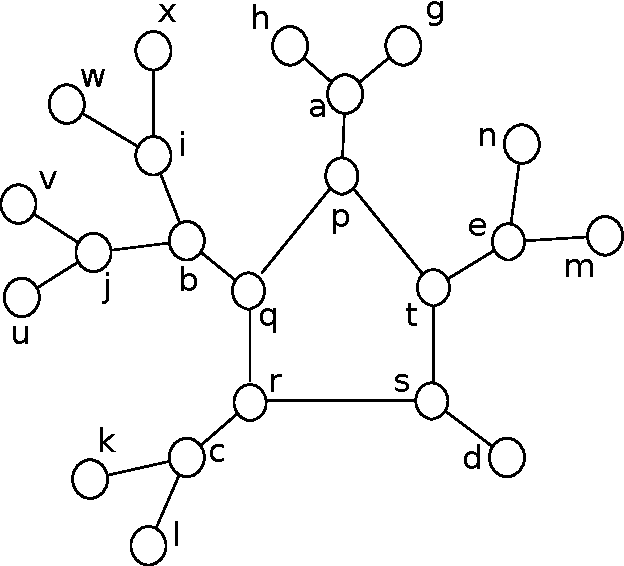
\includegraphics[scale=0.4]{pent} 
%\caption{Pentagon $pqrst$}
%\label{fig:pent}
%\end{center}
%\end{figure}

%\lipsum[1]

%\section{SECTION NAME}
%\lipsum[2]

%\begin{table}
%\centering
%\begin{tabular}{| c | c |}
%\hline
%{\bf item 1} & {\bf item 2} \\ \hline
%
%abcde & 5 \\ \hline
%
%pqrst & 4 \\ \hline
%\end{tabular}
%\caption{A sample table}
%\label{table:1}
%\end{table}


\chapter{System Design}

%Replace \lipsum with text.
% You may have as many sections as you please. This is just for reference.

\section{High Level Design}
%\lipsum[2]
% You may add figures in the following manner.

\begin{figure}[here]
\begin{center}	
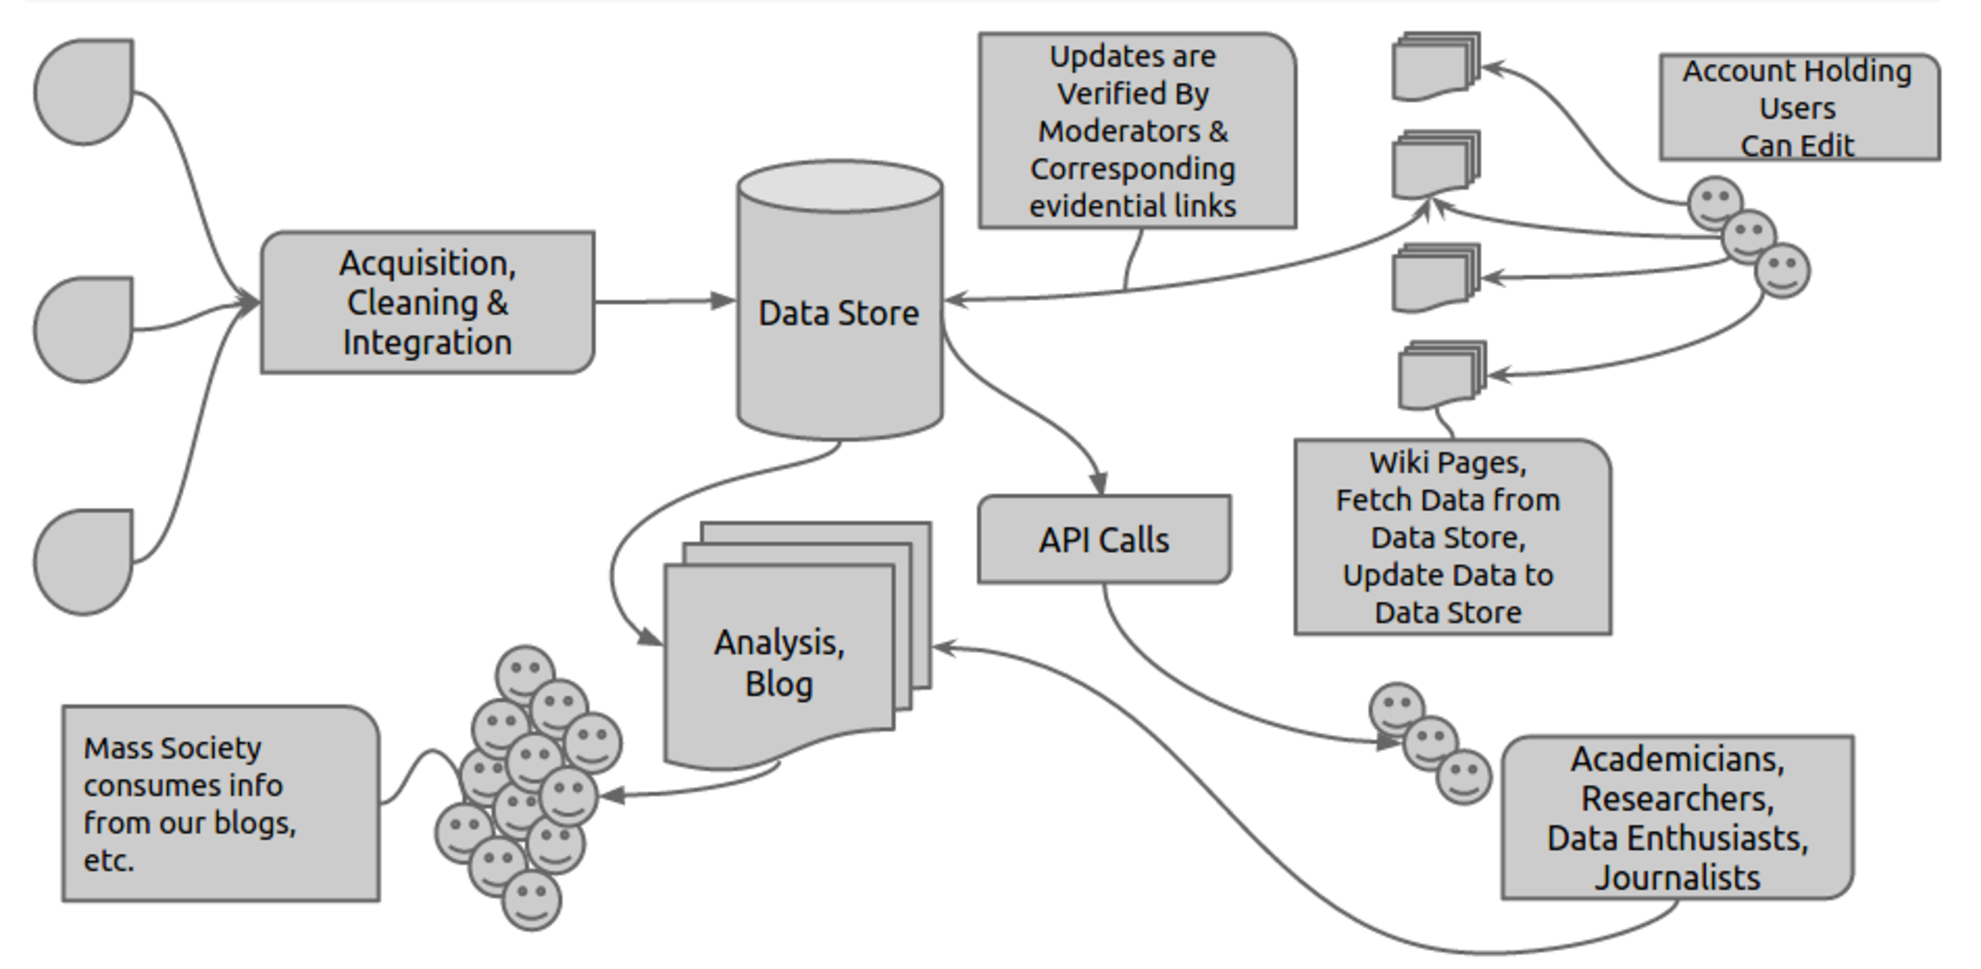
\includegraphics[scale=0.4]{big_pic} 
\caption{Big Picture}
\label{fig:big_pic}
\end{center}
\end{figure}

Above is the generic high level diagram of the entire system as we deduced from our study of the websites above.
We have assumed three main types of users of here:
\begin{enumerate}
\item\textbf{General public} - Use the system for information and news. May also contribute towards data entry.
\item\textbf{Researchers \& Academicians} - Use the site for using social network studies.
\item\textbf{Journalists (Media persons)} - Use the data to frame their news stories.
\end{enumerate}


And keeping these in mind, the system accounts for following functions:
\begin{itemize}
\item\textbf{Data acquisition} - As getting structured data is often difficult system should have a mechanism to automate collection of data from various sources over internet.
\item\textbf{Data Store}  - There should be a central repository for whatever data collected. This repo will store the data in structured form. Care should be taken to keep its integrity, durability and non-redundancy.
\item\textbf{Data Verification} - As the data is sensitive and important, provisions for verification for the input data has to be taken care of. This involves manual labor and system should incorporate this in the entire process.
\item\textbf{Data Visualization} - A portal for the public display of data (in tables, visualizations etc.).
\item\textbf{APIs} - To provide our data for use with other applications.
\end{itemize}

\section{Technical design}
%\lipsum[3]
Accordingly we have incorporated the functionalities in the following way:\\

\begin{figure}[here]
\begin{center}	
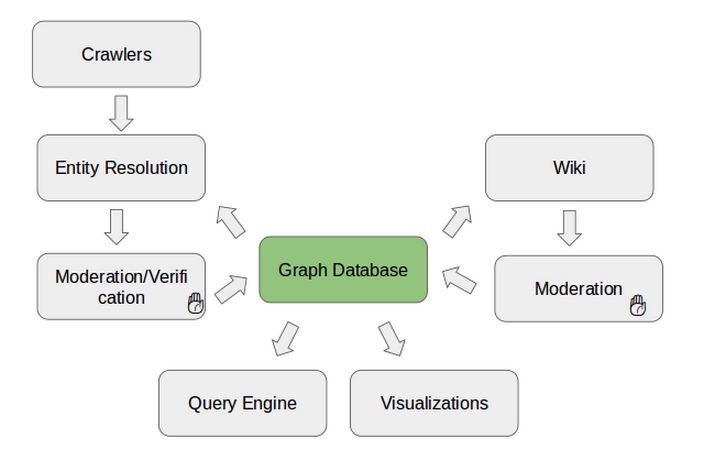
\includegraphics[scale=0.4]{tech_pic} 
\caption{Proposed System}
\label{fig:tech_pic}
\end{center}
\end{figure}

Components include:
\begin{itemize}
\item\textbf{Crawlers-Cleaner-Resolver} - As a part of the data acquisition module, the crawler crawls specific websites and scrapes data in format specified in a static file. Cleaner and resolver works on the scraped data. The cleaner makes the data more structured by keeping all data in specific format, discarding missing values etc. The resolver acts on the data to remove all duplicate entries (and merge similar entries) so to keep the data non redundant as possible.
\item\textbf{Verifier}- The data coming from the crawler after resolution is verified by human moderator. Any to-be-updated information is first human moderated. Any new data is then fed to the graph database.
\item\textbf{Graph database} - Acts as the data store for the system storing structured data with nodes as entities and edges as relationships.
\item\textbf{Web portal(Query Engine, Visualization, Wiki)} - This is the final product that is directly visible to the users. All visualizations (graphical, tabular) are done here. It also has an wiki interface for an end user to add more entities/relations to the graph database. The portal also includes a query/search engine to show results as per specific user queries.
\item\textbf{API} - Registered users can use this to read in data from the datastore in their application.
\end{itemize} 

%\section{SECTION NAME}
%\lipsum[2]


\chapter{System Pipeline}

%Replace \lipsum with text.
% You may have as many sections as you please. This is just for reference.
\begin{figure}[here]
\begin{center}	
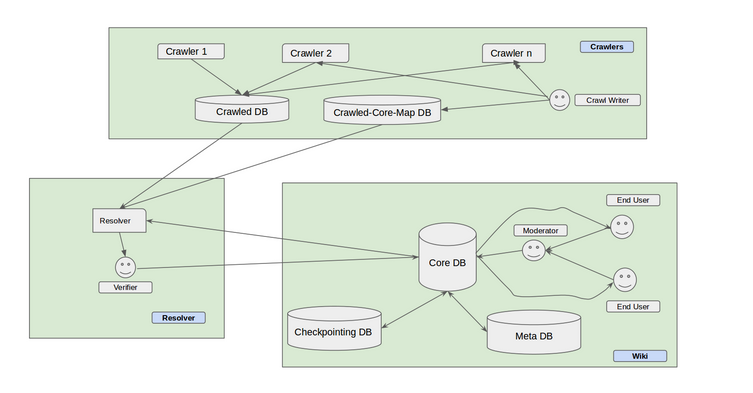
\includegraphics[scale=0.4]{sys_pipeline} 
\caption{System pipeline}
\label{fig:sys_pipeline}
\end{center}
\end{figure}
The total pipeline of the system can be seen in figure above. Overall, we have decomposed the system into 3 cohesive modules. In order of the data flow, they are - 
\begin{quotation}
Crawlers $\rightarrow$ Resolver $\rightarrow$ Wiki
\end{quotation}

\section{Crawlers}
%\lipsum[2]
This is the data acquisition module we have designed. Internally this module consists of the following components:

\subsection{\textbf{Crawler(s)}} - These are basically python scrapy/beautiful soup/selenium scripts to crawl particular websites and srape data from them. The nature of the data (i.e - data types, labels) is mentioned in the \emph{\textbf{Crawled-Core-Map}} database.

\subsection{\textbf{Crawled-Core-Map database}} - Contains the type of the data, its name(or label) to be scraped from a website. This mapping information is used by crawlers to produce output data of specific type,label. This map along with the specific crawlers are written by the developers (\emph{\textbf{Crawl-Writers}})

\subsection{\textbf{Crawled database}} - The raw output from the crawlers is written here. The schema of this database is largely dictated by the \emph{\textbf{Crawled-Core-Map}} database. The data is then read from this database into the \emph{\textbf{Resolver}} module.

\subsection{\textbf{Crawl Writers}} - They are the human components of this module. These persons are developers who write specific scripts to scrape desired websites. They are also responsible for maintaining the data schema in \emph{\textbf{Crawled-Core-Map}} database.



\section{Resolver}
%\lipsum[3]
This module works to fine tune the data scraped by the crawlers. All data collected thus far are mostly unformatted with duplicate or missing values. The function of this module is to process such data into a form suitable for the database.
Its constituents are:


\subsection{\textbf{Resolver}} - It takes the data from the Crawled database as input. The resolver can be further divided into two parts -

\begin{itemize}
\item\textbf{Cleaner} - The cleaner does the text normalization before the actual process for resolving begins. This includes out-of-format data, capitalization, missing-value issues which if not dealt with may cause the resolver to give low accuracy.
\item\textbf{Resolver/Duplicator} - Function of resolver is two-fold. Firstly, it checks any duplicate records in the incoming data (i.e. - data from the crawled database) and removes if any. Then, it resolves the entries from the crawled data with that of the core data. And outputs all possible matchings to the verifier for verification/tagging. 
\end{itemize}

\subsection{\textbf{Verifier}} The authenticity of the data should be checked before it can be inserted into the \emph{\textbf{Core Database}}.  The function of the verifier module and thus the human moderator is to tag the records outputted by the resolver module. These tagged records are the ones which are finally added to the \emph{\textbf{Core Database}}.


\section{Wiki}
This module is the web portal that is directly accessible to the end users. It consists of the interfaces that allow user to view, add, delete entities and their relationships interactively. 

\subsection{\textbf{Core Database}}
This is the main data store of the system. Care has been taken to ensure that whatever data goes in is redundant, free of noise and authenticated. \textbf{Neo4j GraphDB} \cite{Neo4j} is used in the backend for this. 

\begin{itemize}
\item\textbf{Why Graph database preferred here?}\\
Lot of brainstorming went in deciding to use Neo4j graph database. This is because a graph database stores the relations of records in the physical layer (unlike relational database) which makes faster retrieval of connections of entities without joins. And most of the analysis in social networks involves reading in the relationships/connections between entities. Hence query results can be produced faster here without any complicated joins.
\end{itemize}

\subsection{\textbf{Meta Database}} 
This contains the description of the data(format, source, type) being inserted in the database. This is especially useful when the data is authenticated against real-world information, so that every ounce of data in the core database is accounted for.
\subsection{\textbf{Checkpointing Database}}
Without a checkpoint, a Wiki is un-achievable. With every new update, a log of all changes is stored in this database. This is later used to roll back to a previous state to undo any new updates that occured. 
\subsection{\textbf{Web Server}}
Background server that hosts the web application currently has 3 major functions.
\begin{itemize}
\item\textbf{Wiki + Visualization} - The basic functionality of the web application is to provide the users with profiles and connections of organizations and personas which they can edit. The server also maintains a mechanism for checkpointing any data received.
\item\textbf{Query Engine} - To support the queries required for analysis of the network the server implements a query engine which takes queries of specific pattern and return results in tabular or visual format. This is achievable by Cypher query language which facilitates inquiring graph-like queries over Neo4j. These queries would go on the lines like: How are two entities connected? What is the shortest path between two entities? How far an influence of an entity goes over the graph? 
\item\textbf{Read API} - External applications can give GET requests to read data in json format. This aids research and analysis by end users.	
\end{itemize}
\subsection{\textbf{Others}}
Human components in the system - \emph {Users} and \emph{Moderators}. Users include the wiki-users who edit the Wiki to enter any new/updated info they have. They have to provide an evidential link for any information they commit.\\
The job of moderators is to verify records entered by users in the Wiki. They can be experts in their domain, they need to cross-verify from trusted sources.

\section{Example}
%\lipsum[2]
Here we describe how the Verifier and Resolver actually work with a working example.
\subsection{\textbf{Verifier + Resolver}}	
\begin{table}
\centering
\begin{tabular}{| c | c | c |}
\hline
{\bf Name} & {\bf Age } & {\bf Sex }\\
\hline
\end{tabular}
\caption{Sample data formats}
\label{table:1}
\end{table}


\begin{table}
\centering
\resizebox{\columnwidth}{!}{
\begin{tabular}{| c | c | c | c | c | c |}
\hline
{\bf Entity no. } & {\bf Graph label } & {\bf Graph props } & {\bf Mysql props } & {\bf Graph resolve props } & {\bf Mysql resolve props }\\
%1 & person & name,age,sex & name,age,sex & name & name \\
\hline
1 & person & name,age,sex & name,age,sex & name & name \\
\hline
\end{tabular}
}
\caption{Sample record of Crawled-Core-map database}
\label{table:2}
\end{table}

Let us say that the crawler crawls data and saves it in a format like in Table - \ref{table:1}
Also the crawler has an accompanying map-data information which looks like - \ref{table:2}\\
\emph{graph-props} column have one to one order wise mapping with \emph{mysql-props} column.\\
\emph{graph-resolve-props} column have one to one order wise mapping with \emph{mysql-resolve-props} column.\\

So, basically in the crawled data, each row represents a node with label :person and attributes (name, age, sex) in the core database.\\

\begin{enumerate}
\item Now, when a verifier logs-in a row from the \ref{table:1} is fetched, then \ref{table:2} is used to frame a query to search an entity with the name like in the row.
\item Matching nodes are suggested after the query to the verifier.
\item If verifier selects one of the propsed nodes, the resolved node is updated.
\item Else if the verifier doesn't find any matching node, a new node correspoding to the selected row is created and inserted in the core database.
\end{enumerate}

\subsection{\textbf{Wiki + Visualizations }}

\textbf{Profiles}\\

Following is a typical profile in the Wiki-

\begin{figure}[here]
\begin{center}	
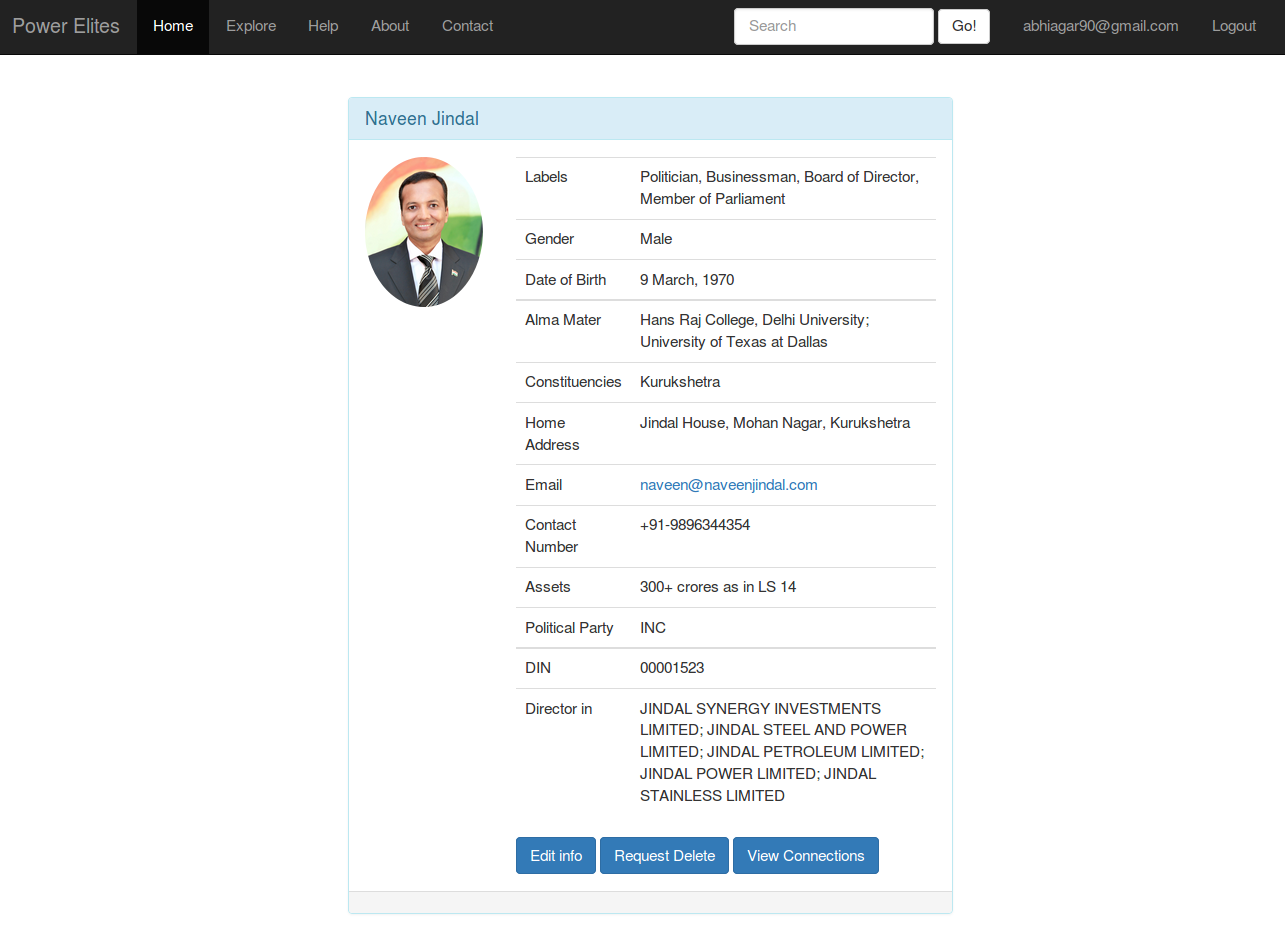
\includegraphics[width=\textwidth]{Jindal} 
\caption{Naveen Jindal Profile}
\label{fig:jindal}
\end{center}
\end{figure}

The figure above shows the Wiki page for industrialist Naveen Jindal containing information about him. It also contains interfaces for any registered user to edit as happens in a Wiki. It also allows the user to show connections of the person.\\

\textbf{Connections (Visualizations)}\\

\begin{figure}[here]
\begin{center}	
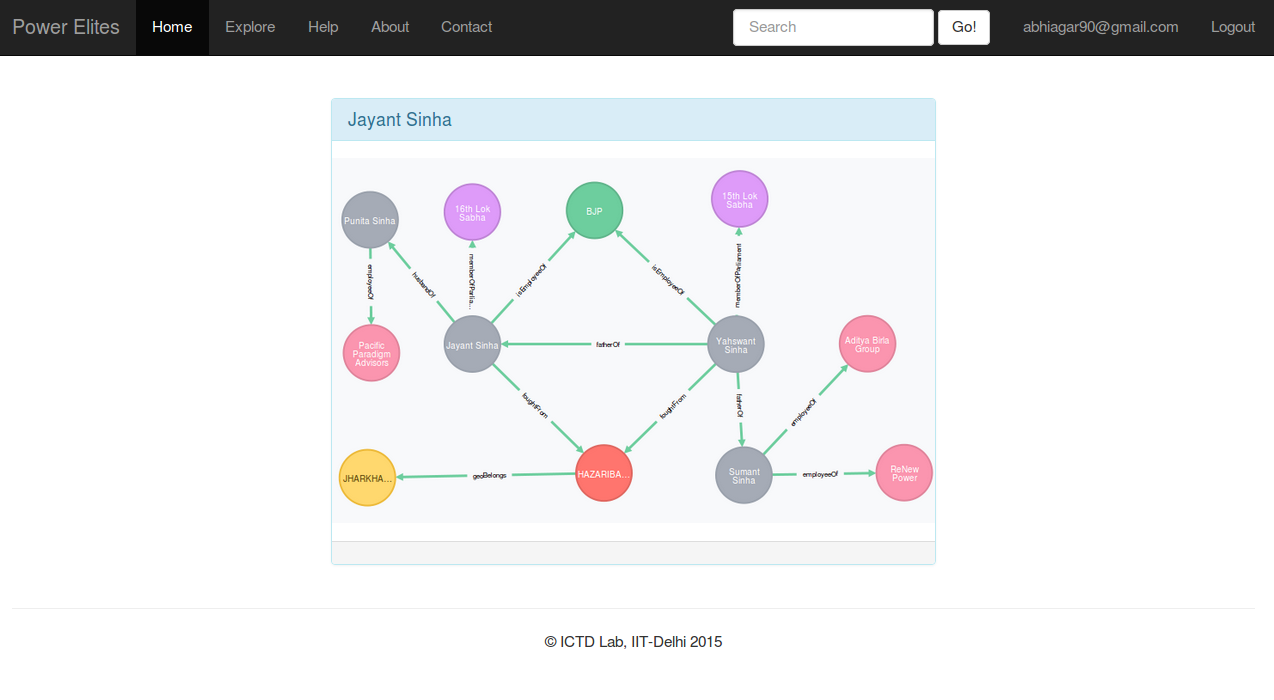
\includegraphics[width=\textwidth]{Sinha} 
\caption{Jayant Sinha Connections}
\label{fig:sinha}
\end{center}
\end{figure}
The figure above shows the connections for Minister of State for Finance Jayant Sinha. His connections include corporates firms like the \textbf{Aditya Birla Group} and \textbf{Pacific Paradigm Advisors} .

Other popular influence networks that our system shows is that of \emph{Gandhi Family and their Corporate linkups}, \emph{Jaydev Galla with his company with a large asset value}, \emph{Kamal Nath with Moser Baer}, \emph{Ravi Shankar Prasad with News 24 channel}.

\begin{figure}[here]
\begin{center}	
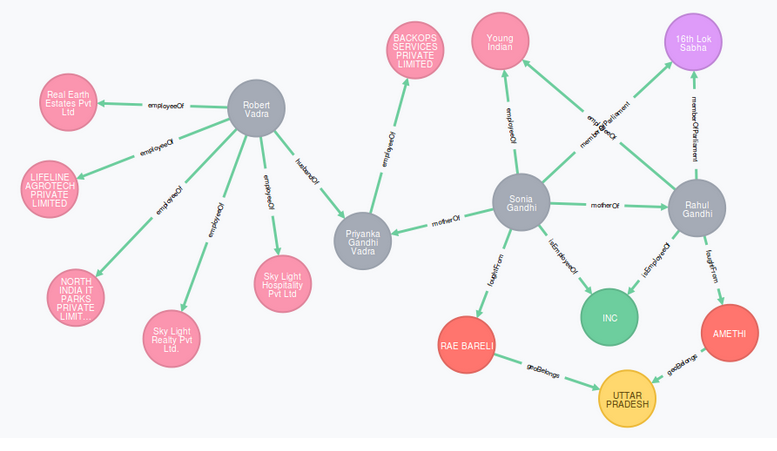
\includegraphics[scale=0.4]{Gandhi} 
\caption{Gandhi family}
\label{fig:gandhi}
\end{center}
\end{figure}

\begin{figure}[here]
\begin{center}	
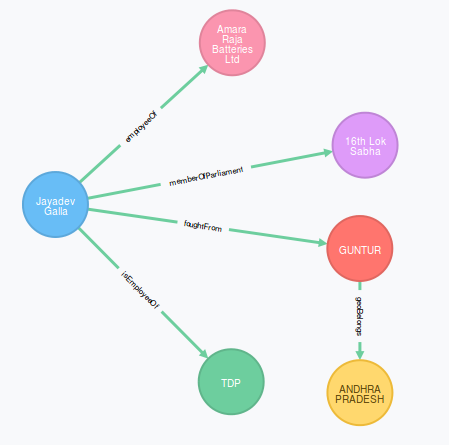
\includegraphics[scale=0.4]{Jaydev} 
\caption{Jaydev Galla Connections}
\label{fig:jaydev}
\end{center}
\end{figure}

\begin{figure}[here]
\begin{center}	
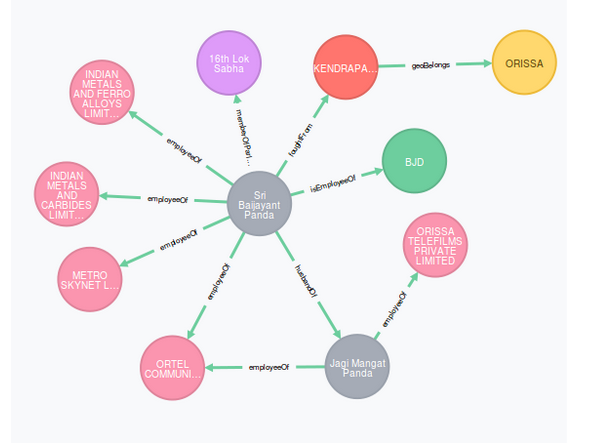
\includegraphics[scale=0.4]{Jay_Panda} 
\caption{Jay Panda Connections}
\label{fig:jaypanda}
\end{center}
\end{figure}

\begin{figure}[here]
\begin{center}	
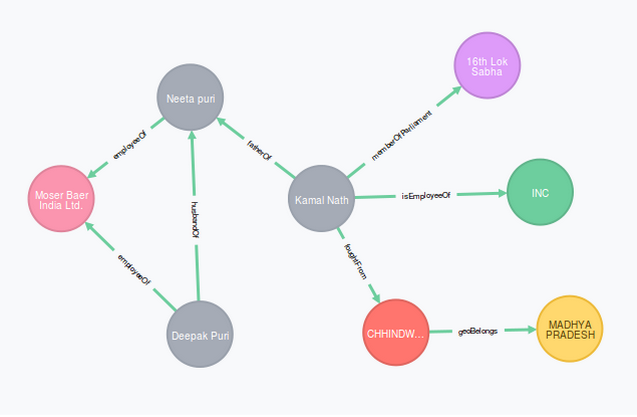
\includegraphics[scale=0.4]{Kamal_Nath} 
\caption{Kamal Nath Connections}
\label{fig:kamalnath}
\end{center}
\end{figure}

\begin{figure}[here]
\begin{center}	
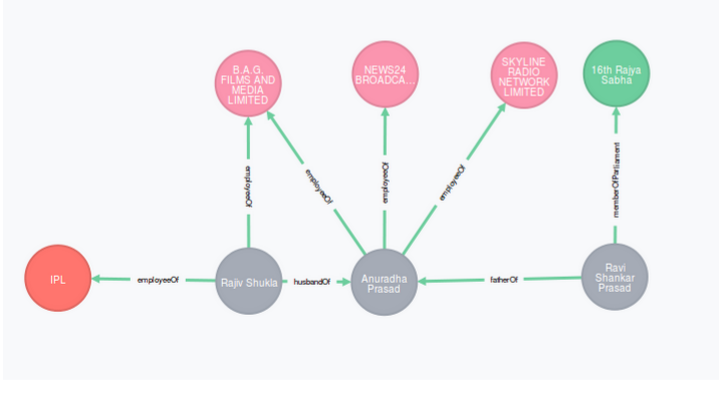
\includegraphics[scale=0.4]{Ravi_Shankar} 
\caption{Ravi Shankar Connections}
\label{fig:ravishankar}
\end{center}
\end{figure}



\chapter{Challenges}

%Replace \lipsum with text.
% You may have as many sections as you please. This is just for reference.

\section{Datasets acquisition}
Biggest challenge in mining political, bureaucratic, corporate data is the difficulty in getting relevant sources and structured information.\\\\
For our initial use cases we began by using political data from \textbf{MyNeta} \cite{MyNeta}. We plan to enrich this data from LokSabha and Rajya Sabha archives.
For corporate data, we used publicly available information from \textbf{CompanyWiki} \cite{CWIKI} and \textbf{Ministry of Corporate Affairs} \cite{MCA}.
As the system progresses we plan to include retired IAS/IPS officers, PPP data, family data of politicians, donations in our growing dataset. We already have about 1000+ politicians, 60000+ business people, 90000+ companies in our current core DB.  

\section{Data Modelling}
After getting some data the challenge was to model the data for the graph database. This would ensure listing of all possible entities and relationships of the system. Care was taken to form such relationships so that in the long run, queries supported by the system take optimum time to produce results.
The prominent entites(nodes) and relationships(links) modelled so far:\\\\
\underline{\textbf{Nodes/Entities}}-\\
(\textbf {Person} (uuid, name, address-location, DOB))\\
(\textbf{Politician} (uuid, name, mynetaid-electionname-year, constituency))\\
(\textbf{Alias} (uuid,name,context))\\
(\textbf{Party}(uuid,name,type:\emph{"national,state,regional"},start-year,HQ))\\
(\textbf{Company}(uuid,cin,name,location,income,expenditure,profit,value))\\
(\textbf{IAS} (uuid,name,DOJ,year,IAS-ID,posting-location))\\
(\textbf{Employee}(uuid,din,name,designation))\\
(\textbf{Govt-Body}(uuid,name,location))\\

\underline{\textbf{Relationships/Links}}-\\
(\textbf{Politician})$\rightarrow$(\textbf{member-of}(id,type,years)$\rightarrow$(\textbf{Party})\\
(\textbf{Politician})$\rightarrow$(\textbf{member-of}(id,type,years)$\rightarrow$(\textbf{Govt-Body})\\
(\textbf{IAS})$\rightarrow$(\textbf{member-of}(id,type,years)$\rightarrow$(\textbf{Govt-Body})\\
(\textbf{Employee})$\rightarrow${employee-of}(id,designation,years)$\rightarrow$(\textbf{Company})\\
(\textbf{Company})$\rightarrow${donated}(id,cin,party,amt,year)$\rightarrow$(\textbf{Party})\\
(\textbf{Person})$\rightarrow${family}(id,is-biological$\rightarrow$(\textbf{Person})\\
(\textbf{Person})$\rightarrow${profession}(id,type)$\rightarrow$(\textbf{Politician})\\
(\textbf{Person})$\rightarrow${profession}(id,type)$\rightarrow$(\textbf{Corporate})\\
(\textbf{Person})$\rightarrow${profession}(id,type)$\rightarrow$(\textbf{IAS})\\
(\textbf{Person})$\rightarrow${aka}(id)$\rightarrow$(\textbf{Alias})\\

\section{Latency and Optimizations}
Although implementation of basic system is ready, its performance suffers when single GET request to the Web server calls for multiple read requests to the core database. We are planning to alleviate this problem by indexing the database to optimize search time, forking multiple threads.


\chapter{Epilogue}
%TODO - expand the questions
\section{Conclusion}
 In short what hypothesis you predicted before starting to build the system?? Do you find them in the results?? Any other interesting patterns?? 
What else can you conclude from your work?? What are your conclusions from the data collection stage? How and why is it difficult to get Indian data?? Did the data model worked well with graph db ?? Is it possible to resolve entities from two different datasets and find interesting connections??  What did your system show after data mashup?? How practical is your system taskflow if deployed in real world??

\section{Future work}
%\lipsum[2]
We have tried to start a process of building a system which in the long run will help the Indian society. Our best efforts were to cover up as much functionality as possible. Yet however, many other problems or features are left to be done in future.
%TODO - expand the questions
\begin{itemize}
\item Scaling up - The designed system works fine. How the system would scale up? How to handle more data when it is fed to the system?
\item Better Visualizations - Can the visualizations be saved/ annotated/ more interacting??
\item Inference Engine - Can the inferencing process be automated? Like in expert systems which uses a knowledge base and Prolog scripts to produce more knowledge??
\item Better analysis of Social Networks - can the different questions about the social graph be answered? What about degree centrality?? No. of weak ties?? Clusters and their strengths? Can we compare with the random graph model to produce some interesting social network behaviors ??
\item Better Query Engine - Can the query engine be improved so that even users not knowing CQL can give queries?
\item Other use cases - Can other data be looked to expand the network with more nodes and relations?? What about IAS officers?? Monetary donations?? Media ownerships??
\end{itemize}


\bibliographystyle{plain}
\bibliography{biblio}

%\appendix
%\chapter{CHAPTER NAME}

\section{SECTION NAME}
\lipsum[1]

\section{SECTION NAME}
\lipsum[2]

\end{document}
	
